\chapter{Elementare Differentialgeometrie}
\section{Raumkurven}
Wir wollen uns in diesem Kapitel genauer mit elementaren Konzepten der Differentialgeometrie befassen. Wir beginnen zunächst einmal mit der Theorie der Raumkurven und deren Eigenschaften. Wir werden sehen, dass die Konstruktion von Kurven bei bekannter Krümmung und Torsion möglich ist. Zuerst wollen wir die  wichtigsten Definitionen die grundlegend für das Verständnis der Theorie der Raumkurven sind einführen.
\begin{defs}
	Sei $c: I \rightarrow \R$ eine nach der Bogenlänge parametrisierte Kurve, also $\norm{T(s)} = \norm{\dot{c}(s)} = 1 \ \forall s \in I$. \\
	Dann gelten die folgenden Aussagen:
\begin{enumerate}
	\item Die Krümmung von $c$ ist $\mathcal{K} = \norm{\dot{T}(s)} = \norm{\ddot{c}(s)}$
	\item Falls $\mathcal{K}(s) \neq 0$ definieren wir den Hauptnormalenvektor $\mathcal{N}$ sowie den Binormalenvektor $\mathcal{B}$ wie folgt:
	\begin{align}
	\mathcal{N}(s) &= \frac{\dot{T}(s)}{\norm{\dot{T}(s)}} = \frac{1}{\mathcal{K}(s)}\cdot\dot{T}(s) \\
		 \mathcal{B}(s) &= T(s) \times \mathcal{N}(s)
	\end{align}
\end{enumerate}
\end{defs}

\begin{bem}
	Das begleitende Dreibein ist nur an Punkten $s \in I$ mit $\mathcal{K}(s) \neq 0$ definiert!
\end{bem}
\begin{figure}[H]
	\centering
	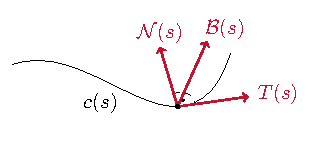
\includegraphics[scale=1.2]{figures/tikz/dreibein.pdf}
	\caption{Visualisierung des begleitenden Dreibeins}
\end{figure}

Wir präsentieren nachfolgend einige fundamentale \textbf{Fakten:}
\begin{enumerate}
	\item $\mathcal{N} \perp T$ und $\dot{T} \perp T$, analog zum 2D-Fall.
	\item $\mathcal{B} \perp T$ und $\mathcal{B}\perp\mathcal{N}$. Außerdem sind die Vektoren normiert: $\norm{T} = \norm{\mathcal{N}} = \norm{\mathcal{B}} = 1$. 
	\item Das Tripel $\left(T(s),\mathcal{N}(s),\mathcal{B}(s)\right)$ bildet eine positiv orientierte Orthonormalbasis des $\R^3$.
	\item $\mathcal{K} \geq 0$.\\
		 Liegt die Kurve $c$ beispielsweise in der $x$-$y$-Ebene, dann ist $\mathcal{K}$ der Betrag der 2D-Krümmung. Demnach ist $\mathcal{K}$ ein Maß dafür, ob $c$ in einer Ebene liegt.
\end{enumerate}
\begin{defs}[Torsion oder Verwindung]
	Wir definieren die Torsion oder auch Verwindung einer Raumkurve wie folgt: 
	\begin{align}
		\tau = \left<\dot{\mathcal{N}}(s),\mathcal{B}(s)\right> 
	\end{align}
\end{defs}

	\begin{itemize}
		\item Die Torsion $\tau$ ist die Größe des Anteils von $\dot{\mathcal{N}}(s)$, welcher aus der $T$-$\mathcal{N}$-Ebene herausragt.
		\item Falls $c$ in der $T$-$\mathcal{N}$-Ebene verläuft, gilt $\tau = 0$ und umgekehrt. 
	\end{itemize}
\begin{satz}[Frenet-Gleichungen]
Die zentralen Gleichungen der Theorie der Raumkurven, die Frenet-Gleichungen haben die folgende Form: 
\begin{align}
	\frac{\dd}{\dd s}\begin{pmatrix} T \\ \mathcal{N} \\ \mathcal{B}\end{pmatrix} = 
	\begin{pmatrix}	
	\phantom{-}0 & \phantom{-}\mathcal{K} & \phantom{-}0 \\
	-\mathcal{K} & \phantom{-}0 & \phantom{-}\tau \\
	\phantom{-}0 & -\tau & \phantom{-}0
	\end{pmatrix}
	\begin{pmatrix} T \\ \mathcal{N} \\ \mathcal{B}\end{pmatrix}
\end{align}
Hier werden $T, \mathcal{N}$ und $\mathcal{B}$ als Zahlen ausgeschrieben.
\end{satz}
\begin{bew}
1. Zeile:
\begin{align*}
\dot{T} = \mathcal{K}\mathcal{N} \quad \text{aus der Definition von $\mathcal{N}$}  	
\end{align*}
2. Zeile: 
\begin{align*}
	0 &= \frac{\dd}{\dd s}\left<\mathcal{N},\mathcal{N}\right> = 2\left<\mathcal{\dot{N}},\mathcal{N}\right>\\
	0 &= \frac{\dd}{\dd s}\left<\mathcal{N},T\right> = \left<\mathcal{\dot{N}},T\right> +\left<\mathcal{N},\dot{T}\right>	\\
	\Rightarrow \left<\mathcal{\dot{N}},T\right> &= -\left<\mathcal{N},\dot{T}\right> = \left<\mathcal{N},\mathcal{K}\mathcal{N}\right> = -\mathcal{K} \\
	\left<\mathcal{\dot{N}},\mathcal{B}\right> &= \tau
\end{align*}
3. Zeile:
\begin{align*}
	\frac{\dd}{\dd s}\left<\mathcal{B},T\right> &= \frac{\dd}{\dd s}\left<\mathcal{B},\mathcal{B}\right> = \frac{\dd}{\dd s}\left<\mathcal{B},\mathcal{N}\right> = 0 \\
	\Rightarrow \left<\mathcal{\dot{B}},T\right> &= -\left<\mathcal{B},\dot{T}\right> = -\left<\mathcal{B},\mathcal{K}\mathcal{N}\right> = 0 \\
	\left<\mathcal{\dot{B}},\mathcal{N}\right> &= - \left<\mathcal{B},\mathcal{\dot{N}}\right> = -\tau
\end{align*}
\end{bew}
Auch hier erlauben wir uns einige \textbf{Bemerkungen:}
\begin{itemize}
	\item $\mathcal{B}$ ist senkrecht zur Schmiegeebene $\operatorname{span}\left\{\mathcal{N},T\right\}$ an $c$.
	\item Taylorentwicklung von $c$ um $s_0 \in I$ liefert:
	\begin{align*}
	c(s) &= c(s_0)	+ (s-s_0)\dot{c}(s_0) + \frac{(s-s_0)^2}{2}\ddot{c}(s_0) + \mathcal{O}((s-s_0)^3) \\
	     &= c(s_0) + (s-s_0)T(s_0) + \frac{(s-s_0)^2}{2}\mathcal{K}(s_0)\mathcal{N}(s_0) + \mathcal{O}((s-s_0)^3)
	\end{align*}
	\item $c$ berührt die Tangente in $s_0$ in 1. Ordnung, $\mathcal{K}$ beschreibt die Änderungsrate des Tangentialvektors.
	\item $c$ berührt die Schmiegeebene in $s_0$ in 2. Ordnung, $\tau$ beschreibt die Änderungsrate der Schmiegeebene. 
\end{itemize}
\begin{satz}[Hauptsatz der Kurventheorie]
	Seien $b>0$, $\mathcal{K}: [0,1]\rightarrow \R, \tau: [0,b]\rightarrow \R$ mit $\mathcal{K}(s)>0 \ \forall s \in [0,b]$ und $c_0, T_0, \mathcal{N}_0 \in \R^3$ mit $\norm{T_0} = \norm{\mathcal{N}_0} = 1$ sowie $T_0 \perp \mathcal{N}_0$ gegeben. \\
	Dann existiert genau eine nach Bogenlänge parametrisierte Kurve $c:[0,b]\rightarrow\R^3$ mit Krümmung $\mathcal{K}$, Torsion $\tau$ und $c(0) = \xi_0$, $\dot{c}(0) = T_0$ sowie $\ddot{c}(o) = \mathcal{K}(0)\mathcal{N}_0$.
\end{satz}
\begin{bew}
Sei 
\begin{align}
K(s)= \begin{pmatrix}	
	\phantom{-}0 & \phantom{-}\mathcal{K}(s) & \phantom{-}0 \\
	-\mathcal{K}(s) & \phantom{-}0 & \phantom{-}\tau(s) \\
	\phantom{-}0 & -\tau(s) & \phantom{-}0
	\end{pmatrix}\tag{$\star$}	
\end{align}
Dann existiert genau eine differenzierbare Funktion $F: [0,b]\rightarrow \R^{n \times n}$ mit $\dot{F} = K$ sowie
\begin{align*}
F(0)=\begin{pmatrix}
	T_0 \\ \mathcal{N}_0 \\ T_0 \times \mathcal{N}_0 \end{pmatrix}
\end{align*}

Dies folgt aus dem Existenz- und Eindeutigkeitssatz von Lösungen linearer Differentialgleichungen. Es gilt:
\begin{align*}
	\frac{\dd}{\dd s} F F^{\mathsf{T}} &= \dot{F}(s) F(s)^{\mathsf{T}} + F(s) \dot{F}(s)^{\mathsf{T}}\\
	&= K(s)F(s)F(s)^{\mathsf{T}} + F(s)F(s)^{\mathsf(T)}K(s)^{\mathsf{T}} 
\end{align*}
Damit erhalten wir mit $X(s) = F(s)F(s)^{\mathsf{T}} $ die eindeutige Lösung der Differentialgleichung:
\begin{align*}
	\dot{X} = KX + XK^{\mathsf{T}}
\end{align*}
mit $X(0) = F(0)F(0)^{\mathsf(T)} = \mathds{1}$. \\

Aber $X(S) = \mathds{1}$ ist auch eine Lösung von $\dot{X} = KX + XK^{\mathsf{T}}$, weil $K + K^{\mathsf{T}} = 0$. \\

Daraus folgt: $\mathds{1} = F(s)F(s)^{\mathsf{T}}$. Außerdem wissen wir dadurch: $\operatorname{det}(F(s)) \in \left\{-1, +1\right\}$. \\
Für die Stetigkeit benutzen wir 
\begin{align*}
\operatorname{det}(F(s)) = \operatorname{det}(F(0)) = \mathds{1} \Rightarrow F(s) \in \operatorname{SO}(3) \ \ \forall s \in [0,b]
\end{align*}
Seien $T, \mathcal{N}$ und $\mathcal{B}$ die Komponenten von $F$, also $F=\left(T,\mathcal{N},\mathcal{B}\right)^{\mathsf{T}}$. 
Sei $c(s) = c_0 + \int_0^s T(t) \dd t$. \\
Sei $(T',\mathcal{N}',\mathcal{B}')$ das begleitende Dreibein von $c$.
\begin{itemize}
	\item $T'(s) = \dot{c}(s) = T(s)$.
	\item $\mathcal{K}(s) = \norm{\dot{T}'(s)}= \norm{\dot{T}(s)} = \norm{\mathcal{K}(s)\mathcal{N}(s)} = \abs{\mathcal{K}(s)} = \mathcal{K}(s)$.
	\item $\mathcal{N}'(s) = \frac{1}{\mathcal{K}'(s)}\cdot\dot{T}'(s) = \frac{1}{\mathcal{K}(s)} \cdot T(s) \overset{(\star)}{=} \frac{1}{\mathcal{K}(s)}\mathcal{K}(s)\mathcal{N}(s) = \mathcal{N}(s)$.
	\item $\mathcal{B}'(s) = T'(s) \times \mathcal{N}'(s) = T(s) \times \mathcal{N}(s)$, weil $\left(T,\mathcal{N},\mathcal{B}\right)$ positiv orientierte ONB ist.
	\item $\tau'(s) = \left<\dot{\mathcal{N}}'(s),\mathcal{B}'(s)\right> = \left<\dot{\mathcal{N}}(s),\mathcal{B}(s)\right> = \left<-\mathcal{K}(s)T(s)+\tau(s)\mathcal{B}(s),\mathcal{B}(s)\right> = \tau(s)$
	\item $c(0) = c_0, \dot{c}(0) = T(0), \ddot{c}(0) = \dot{T}'(0) =\dot{T}(0) = \mathcal{K}(0)\mathcal{N}(0)= \mathcal{K}(0)\mathcal{N}_0$
\end{itemize}




Es bleibt noch die Eindeutigkeit zu zeigen: \\

Die Kurve $c$ ist eindeutig bestimmt durch $c_0$ und $T$ und $T$ sowie $\mathcal{N}$ und $\mathcal{B}$ sind eindeutig durch $T_0$, $\mathcal{N}_0$, $\mathcal{B}_0$ und die Frenet-Gleichungen festgelegt.
\end{bew}


Wir wollen die neuen Konzepte auf \textbf{höhere Dimensionen} verallgemeinern:\\
\begin{defs}[Frenet-Kurven]
	Eine Kurve $c: I \rightarrow \R^n$ heißt Frenet-Kurve, wenn $\dot{c}, \ddot{c}, c^{(3)} \dots c^{(n-1)}$ an jedem Punkt in $I$ linear unabhängig sind. \\
	In drei Dimensionen bedeutet das, dass für alle Frenet-Kurven die Krümmung $\mathcal{K} \neq 0 \ \ \forall s \in I$ ist. Das begleitende $n$-Bein $e_1,\dots,e_n: I \rightarrow \R^n$ erhält man mithilfe des Gram-Schmidt-Verfahrens für $\dot{c}, \ddot{c}, c^{(3)} \dots c^{(n-1)}$: 
	\begin{align}
		e_i = \frac{c^{(i)}-\sum_{j=1}^{i-1}\left<c^{(i)},e_j\right>e_j}{\norm{c^{(i)}-\sum_{j=1}^{i-1}\left<c^{(i)},e_j\right>e_j}}
	\end{align} 
$e_n$ ist der eindeutige Vektor der $e_1(s)\dots,e_n(s)$ zu einer positiv orientieren Orthonormalbasis macht. \\
Die Frenet-Krümmungen $\mathcal{K}_i$ lauten:
\begin{align}
	\mathcal{K}_i(s) = \left<e_1(s),\dots,e_{i+1}(s)\right>
\end{align}
Es gelten die $n$-dimensionalen Frenet-Gleichungen:
\begin{align}
	\frac{\dd}{\dd s}\begin{pmatrix} e_1 \\ \vdots \\ e_n\end{pmatrix} = 
	\begin{pmatrix} 
\phantom{-}0 & \phantom{-}\kappa_1 & \phantom{-}0 & \phantom{-}\ldots & \phantom{-}\ldots & \phantom{-}0 \\ 
-\kappa_1 & \phantom{-}0 & \phantom{-}\kappa_2 & \phantom{-}0 & \phantom{-}\ldots & \phantom{-}\vdots \\ 
\phantom{-}0 & -\kappa_2 & \phantom{-}0  & \phantom{-}\ddots & \phantom{-}\ddots & \phantom{-}\vdots \\
\phantom{-}\vdots & \phantom{-}0 & \phantom{-}\ddots  & \phantom{-}\ddots & \phantom{-}\ddots & \phantom{-}0 \\
\phantom{-}\vdots & \phantom{-}\vdots & \phantom{-}\ddots  & \phantom{-}\ddots & 0 & \phantom{-}\kappa_{n-1} \\
\phantom{-}0 & \phantom{-}\ldots & \phantom{-}\ldots  & \phantom{-}0  & -\kappa_{n-1} & \phantom{-}0
\end{pmatrix}
	\begin{pmatrix} e_1 \\ \vdots \\ e_n\end{pmatrix}
\end{align}
Es gilt außerdem der Hauptsatz der Kurventheorie: \\
Gegeben $\mathcal{K}_1,\dots,\mathcal{K}_{n-1}: I \rightarrow \R$, \ $\mathcal{K}_1,\dots,\mathcal{K}_{n-1} > 0 $ sowie die positiv orientierte Orthonormalbasis $\left(e_1^0,\dots,e_n^0\right)$. \\
Dann existiert genau eine Frenet-Kurve $c: I\rightarrow \R^n$ mit zugehörigen Frenet-Krümmungen $(\mathcal{K}_i)_{i=1,\dots,n-1}$ und dem Frenet-$n$-Bein $(e_1^0,\dots,e_0^n)$ an der Stelle $0 \in I$.
\end{defs}